\chapter{The spatial-diversity framework}
\label{ch:sdframework}
\section{Improving scheduling with spatial-diversity}

In the previous chapter have been addressed the scheduling of jobs of variable size in relation to their probability distribution. Then, there were presented two attempts to approximate the optimal LAS and SRPT schedulers by leveraging multiple priority queues at network interfaces. However, one limitation of this approach remains the scarce number of such priority queues available in commodity switches. In particular, it was mentioned that a large number of priority levels is demanded to better approximate the reference scheduling disciplines, in which $N \rightarrow \infty$ (Sec. \ref{sec:las}). Unfortunately, devices in modern DCNs are usually equipped with no more than 8 priority queues per port, whose majority are reserved for other purposes, like isolating different types of traffic. Indeed, several transport protocols may coexist in the same network, without necessarily being designed to be fair with respect to each other. Example of such transports are RDMA \cite{rdma}, DCTCP \cite{dctcp}, standard TCP and UDP. For this reason, it is realistic to assume having at most $N=2$ priority queues in practical cases. \\
Upon this understanding, the main proposal of this work is to evaluate the possibility of exploiting the high degree of path diversity typically offered by DCN topologies, in order to improve the effectiveness of flow scheduling. Large DCN topologies usually are multilayer recursive Clos networks which offer a variety of equal-cost paths between racks. Precisely, in the simplest 2-layer Fat-Tree there are a number of paths proportional to the number of spines $K$ (Sec. \ref{sec:topology}). The key observation is that much like priority queues, different paths yet are a way for augmenting the granularity of prioritization and for separating flows with different QoS requirements. The novel paradigm being investigated aims to exploit \emph{spatial-diversity} to derive extra priorities and overcome the limitations in the maximum number of available PQs imposed by a single switch. Indeed, the mechanism of priority demotion, as proposed in PIAS, only shifts long flows across PQs of a single interface. Instead, we argue that the same demotion could be potentially applied at DC-level. Consider a Leaf-Spine topology and focus on a single ToR switch (Fig.\ref{fig:sd-key-idea}). The interfaces from such a ToR towards all spines can be seen jointly as a unique big interface with $K$ times more priority queues than a port alone.
\begin{figure}
	\centering
	\begin{subfigure}[htpb]{0.3\textwidth}
		\centering
		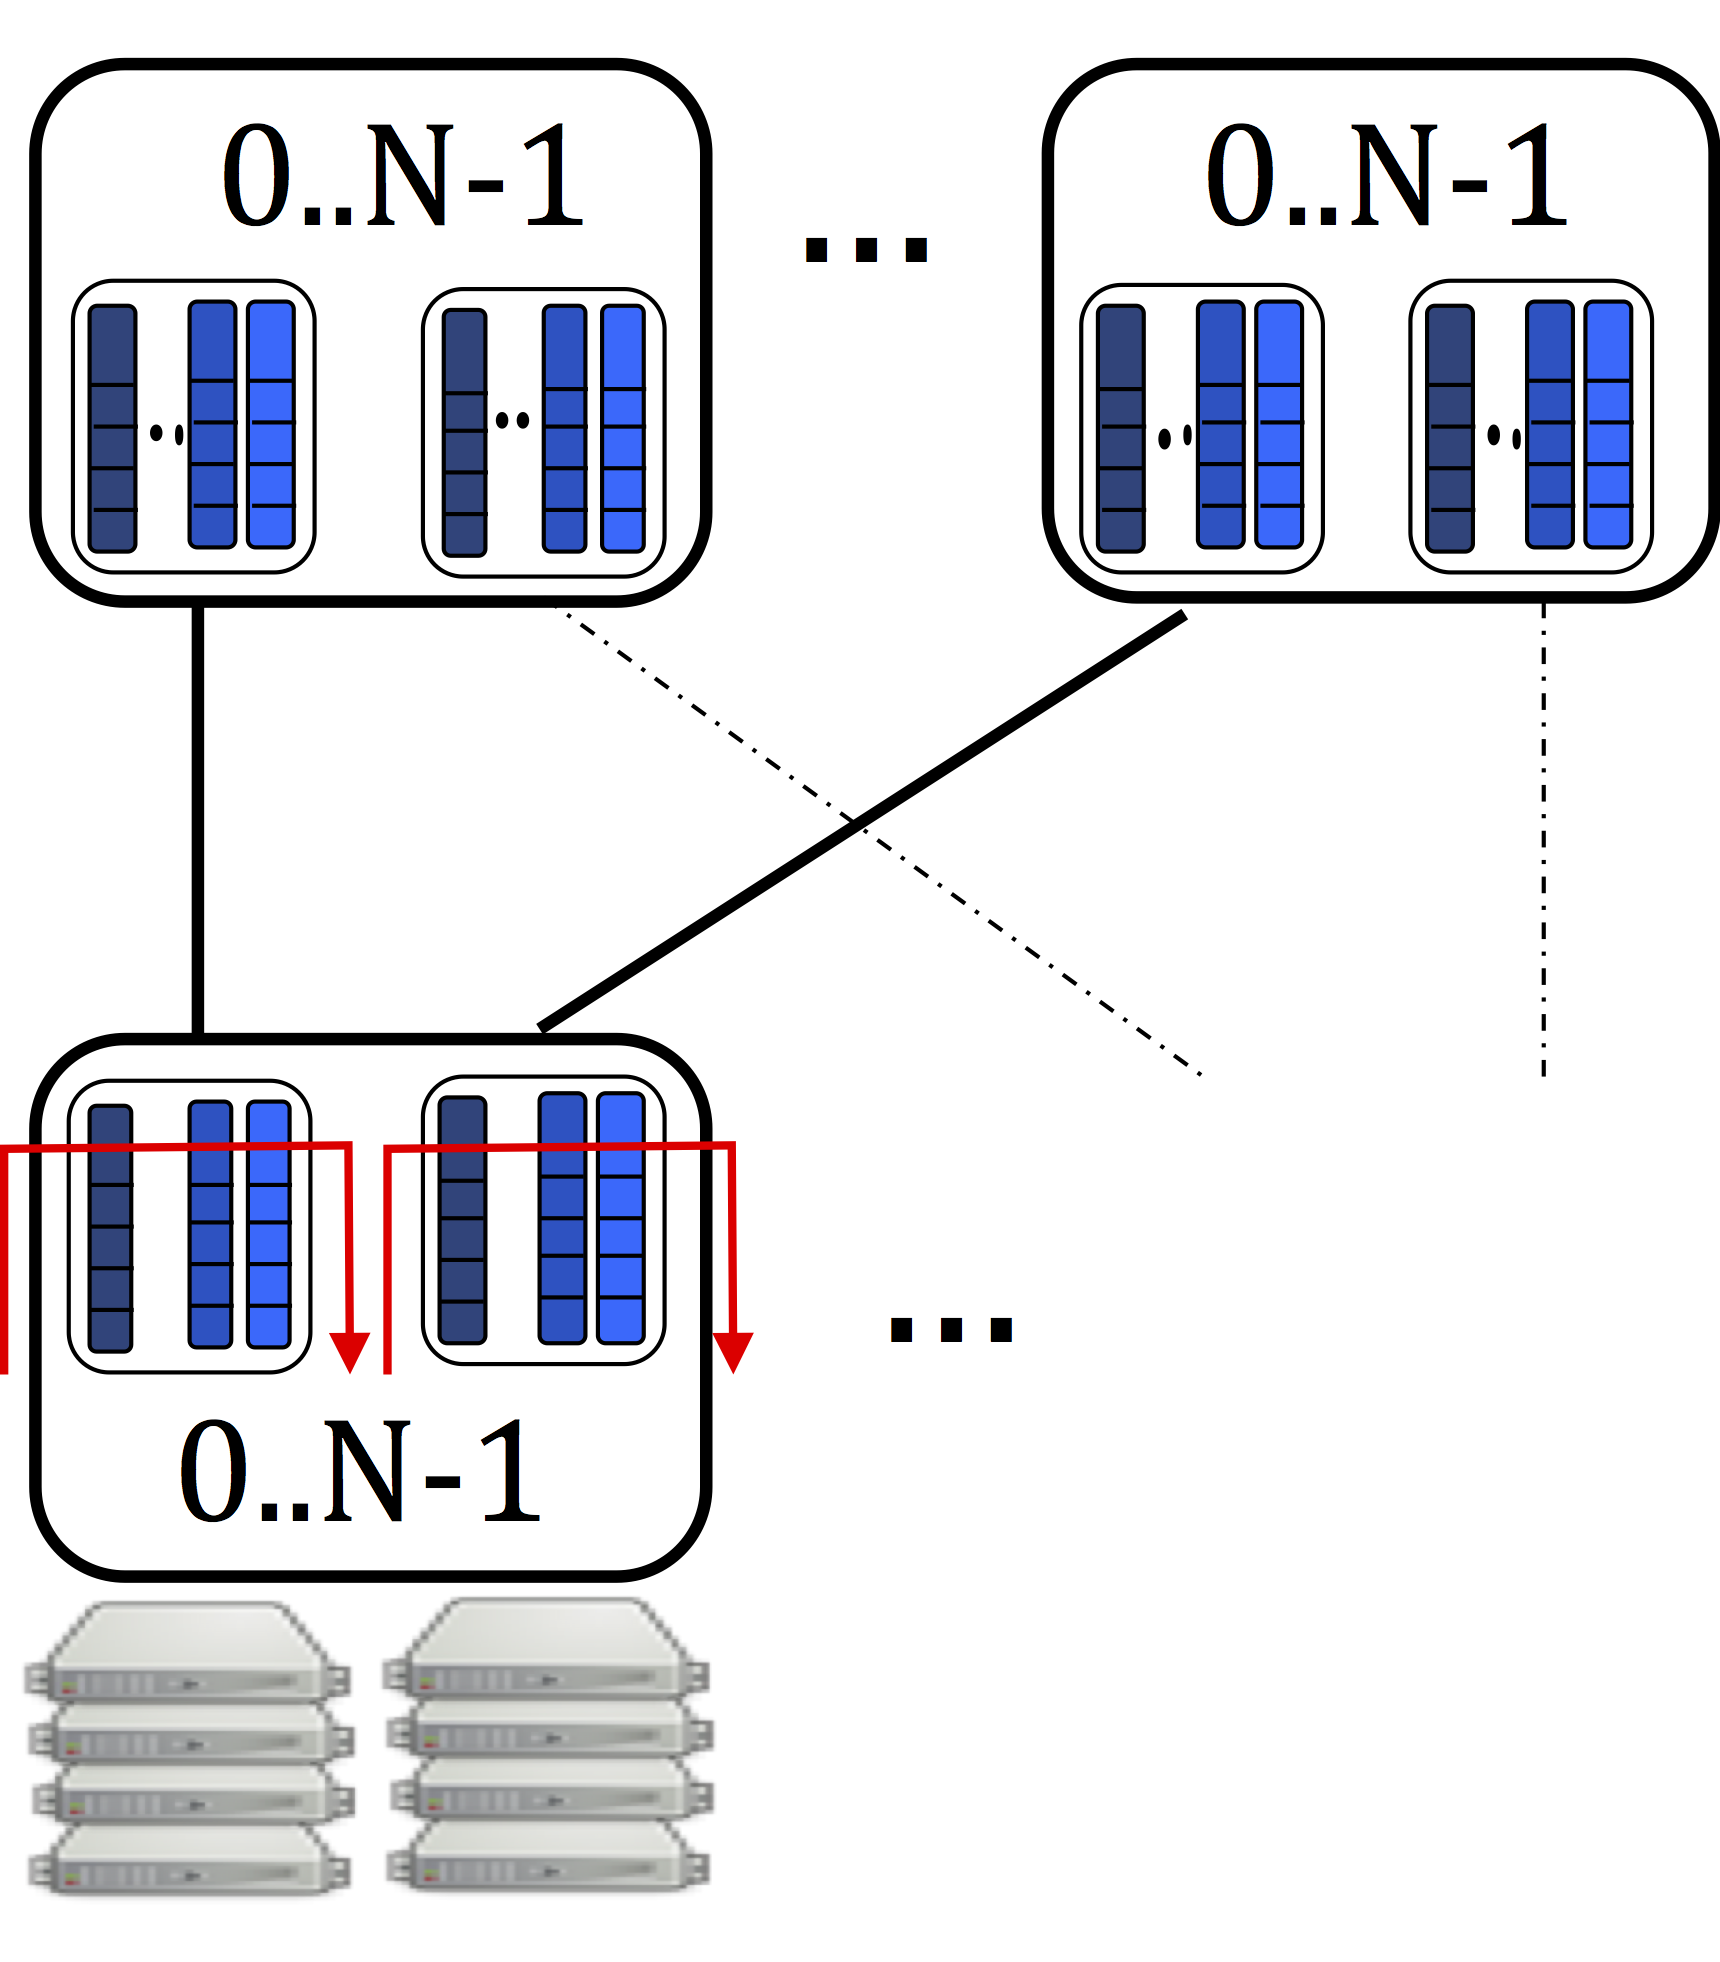
\includegraphics[width=\textwidth]{Chapter2/Figures/mlfq}
		\caption{MLFQ}
		\label{fig:sd-key-idea-mlfq}
	\end{subfigure}
	\hspace{0.2\textwidth}%
	\begin{subfigure}[htpb]{0.3\textwidth}
		\centering
		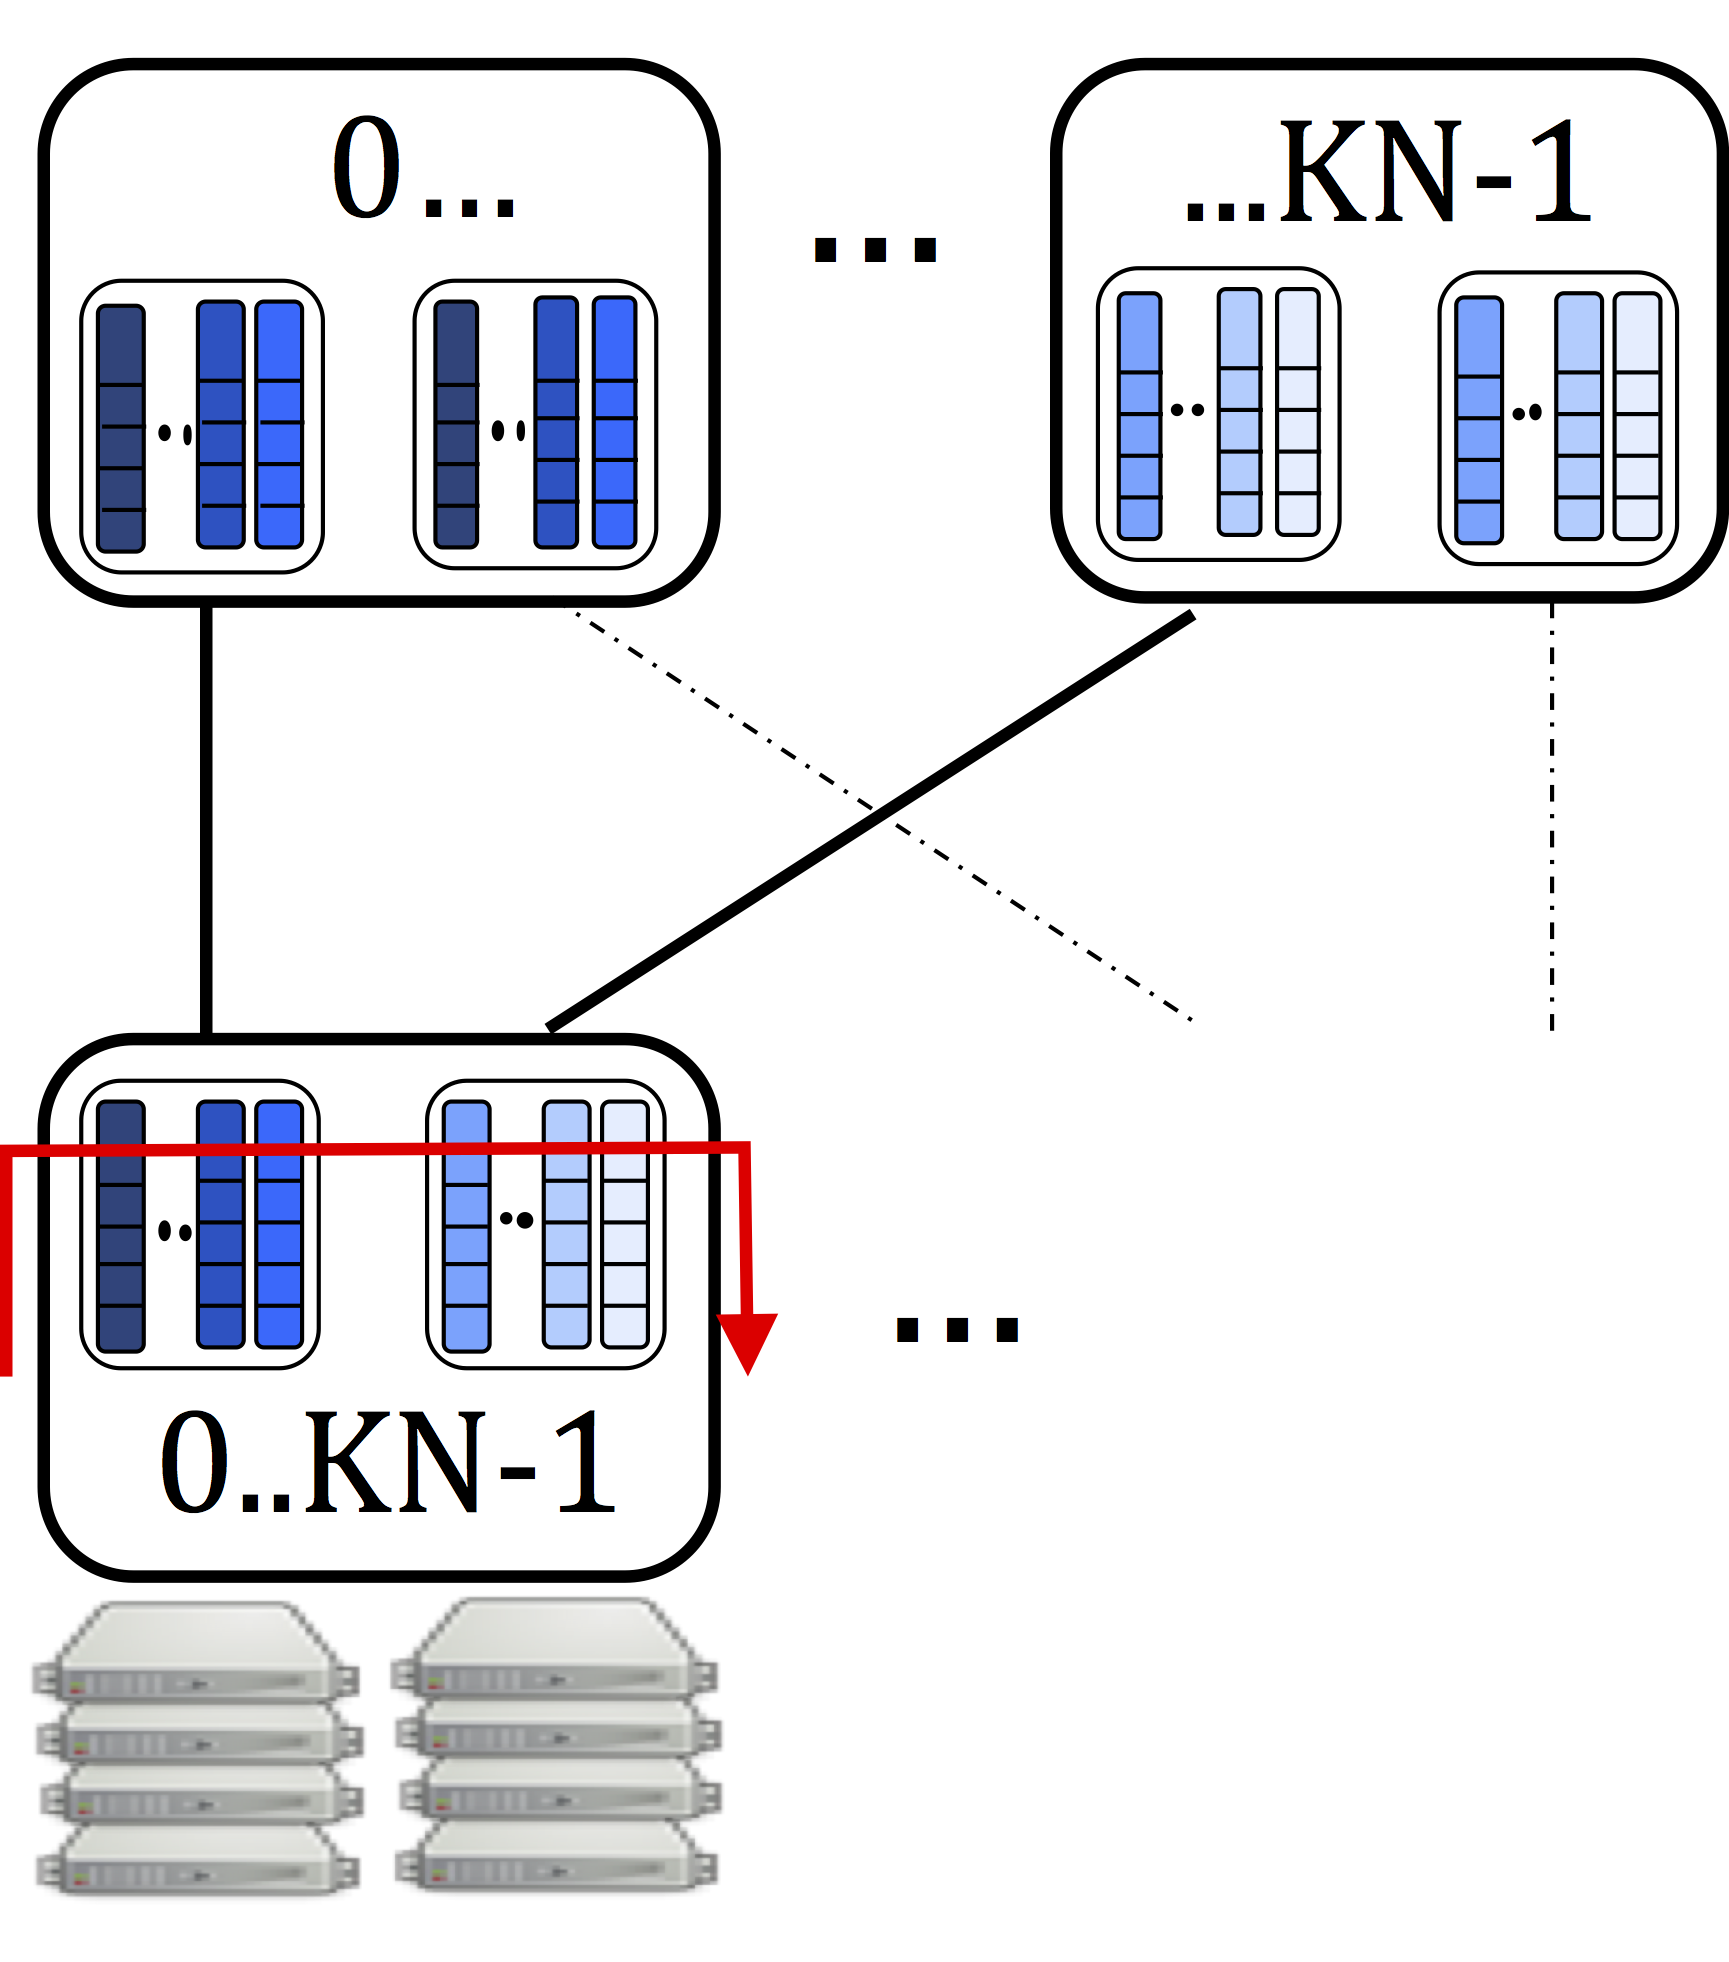
\includegraphics[width=\textwidth]{Chapter2/Figures/sdmlfq}
		\caption{SD-MLFQ}
		\label{fig:sd-key-idea-sdmlfq}
	\end{subfigure}
	\caption{Demotion extension with spatial diversity. Red arrows indicate demotion trajectory of the longest flow. On each switch is reported the priorities it handles. Lower indexes (and darker colors) correspond to higher priorities.}
	\label{fig:sd-key-idea}
\end{figure}
%Differently from 
The basic MLFQ (Fig.\ref{fig:sd-key-idea-mlfq}) focuses on the links individually and thanks to demotion moves flows, during their lifetime, across priority queues of single interfaces. Therefore, every interface handle the same priorities and flows are load balanced on different links independently from the prioritization mechanism. A standard technique for load balancing at flow-level is ECMP, which derives the next hop from the transport-layer tuple \texttt{\{IP ADDRESSES, PORTS, PROTOCOL ID\}}. Instead, our solution in Fig. \ref{fig:sd-key-idea-sdmlfq} --- which we call Spatially-Diverse MLFQ (SD-MLFQ) --- takes advantage of spatial diversity to extend the number of demotion levels beyond the limitation imposed by the PQs on a single interface. Interfaces from any ToR to the connected spines are virtually aggregated to offer a wider range of demotion levels. \\
One new aspect of this novel approach is that a demotion could imply shifting a flow from one path to another of equal-cost. In that light, the routing --- thus load balancing --- over the switching fabric is not blind to the prioritization machinery, but does depend on it. In general, a flow is moved both across queues and spines, effectively allowing a global resource exploitation for the demotion scheme. In order to have a clear and direct notation, the spines are labeled with the priorities handled by their interfaces. Notably, since the demotions that imply a spatial re-route take place at ToRs, all the interfaces on the same spine handle the same priorities. Hence, it is enough a single labeling per spine, valid for all its interfaces. 
A clear benefit of spatial diversity is that finer granularity in priorities is achieved even with few queues per port, at the price of a very limited implementation complexity. Also, elephant flows are better segregated from mice flows, as after a while they are physically moved to different paths inside the switching fabric. Despite its simplicity, relevant works exploring this solution in the field of data center networks seem to be lacking. 

\subsection{Abstraction as queuing system}
\label{sec:threesystemcomparison}
%in the initial phase and get a first glance about its effectiveness
To tackle the spatial diversity framework from a conceptual perspective, three queuing systems are compared. They are shown in Fig.\ref{fig:three-system-comparison}. 
\begin{figure}
	\centering
	\begin{subfigure}[b]{0.3\textwidth}
		\centering
		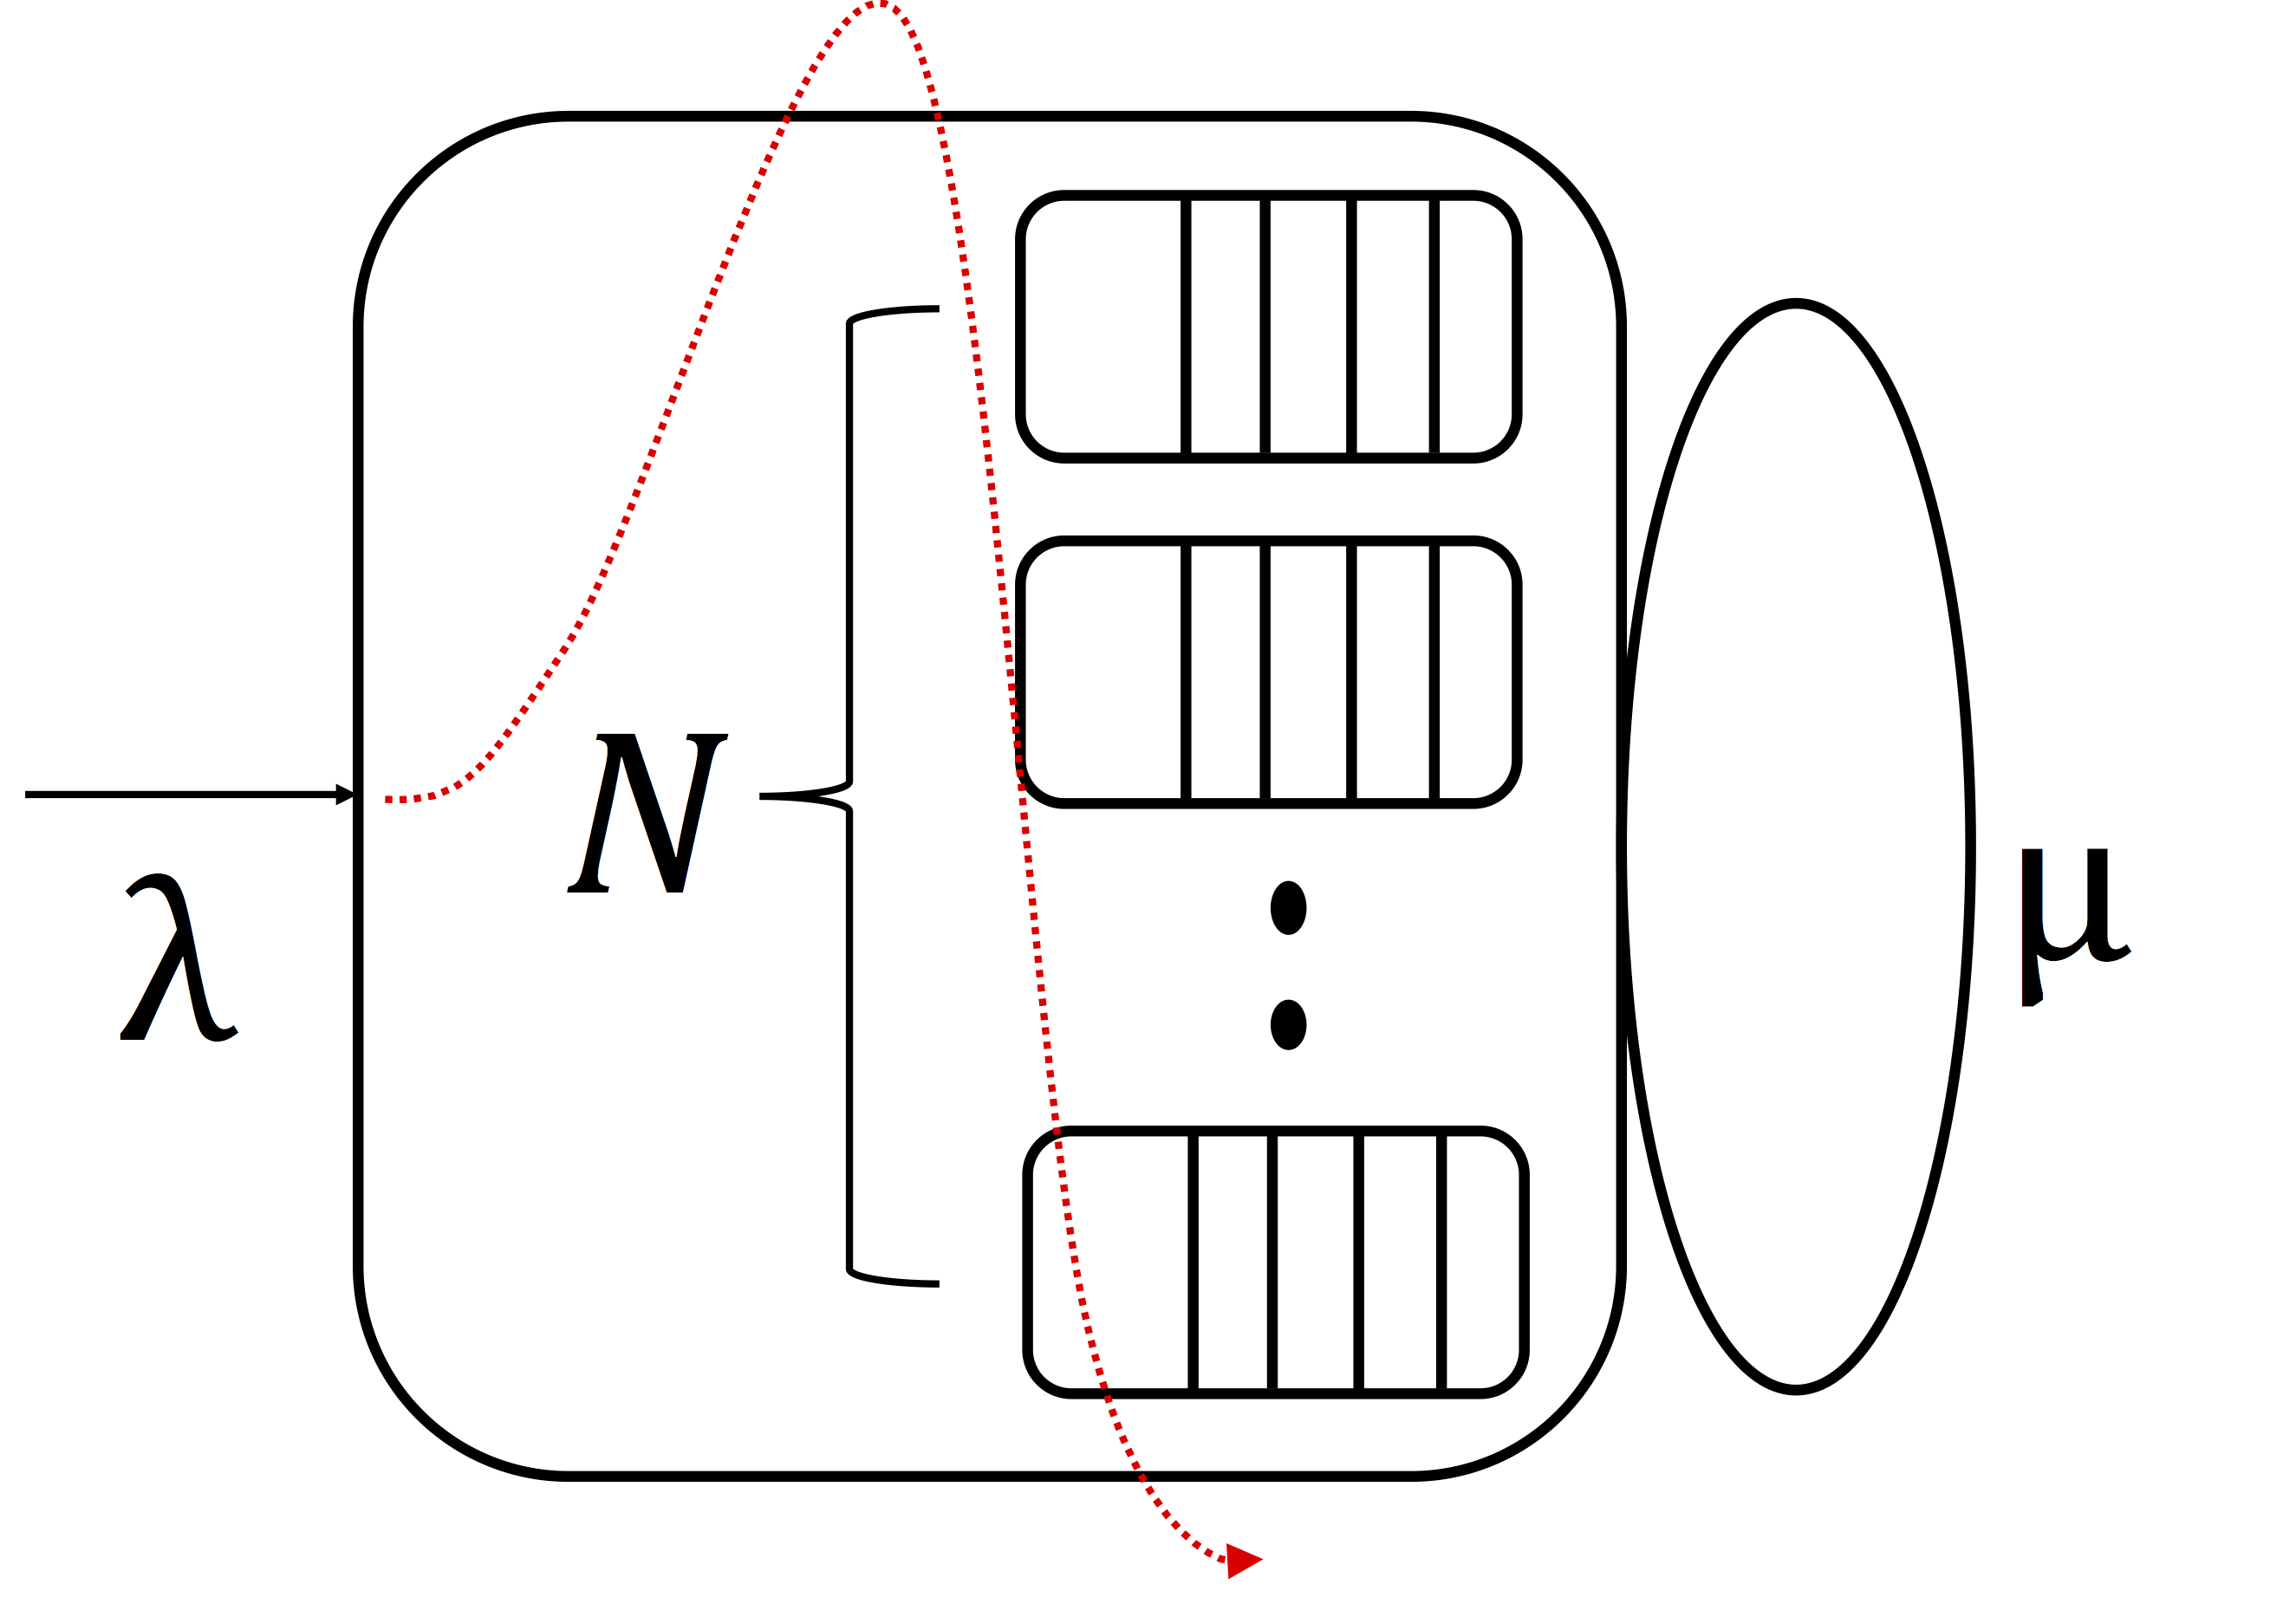
\includegraphics[width=\textwidth]{Chapter3/Figures/switchone}
		\smallskip
		\caption{Super-Server}
		\label{fig:switchone}
	\end{subfigure}
	\hfill
	\begin{subfigure}[b]{0.3\textwidth}
		\centering
		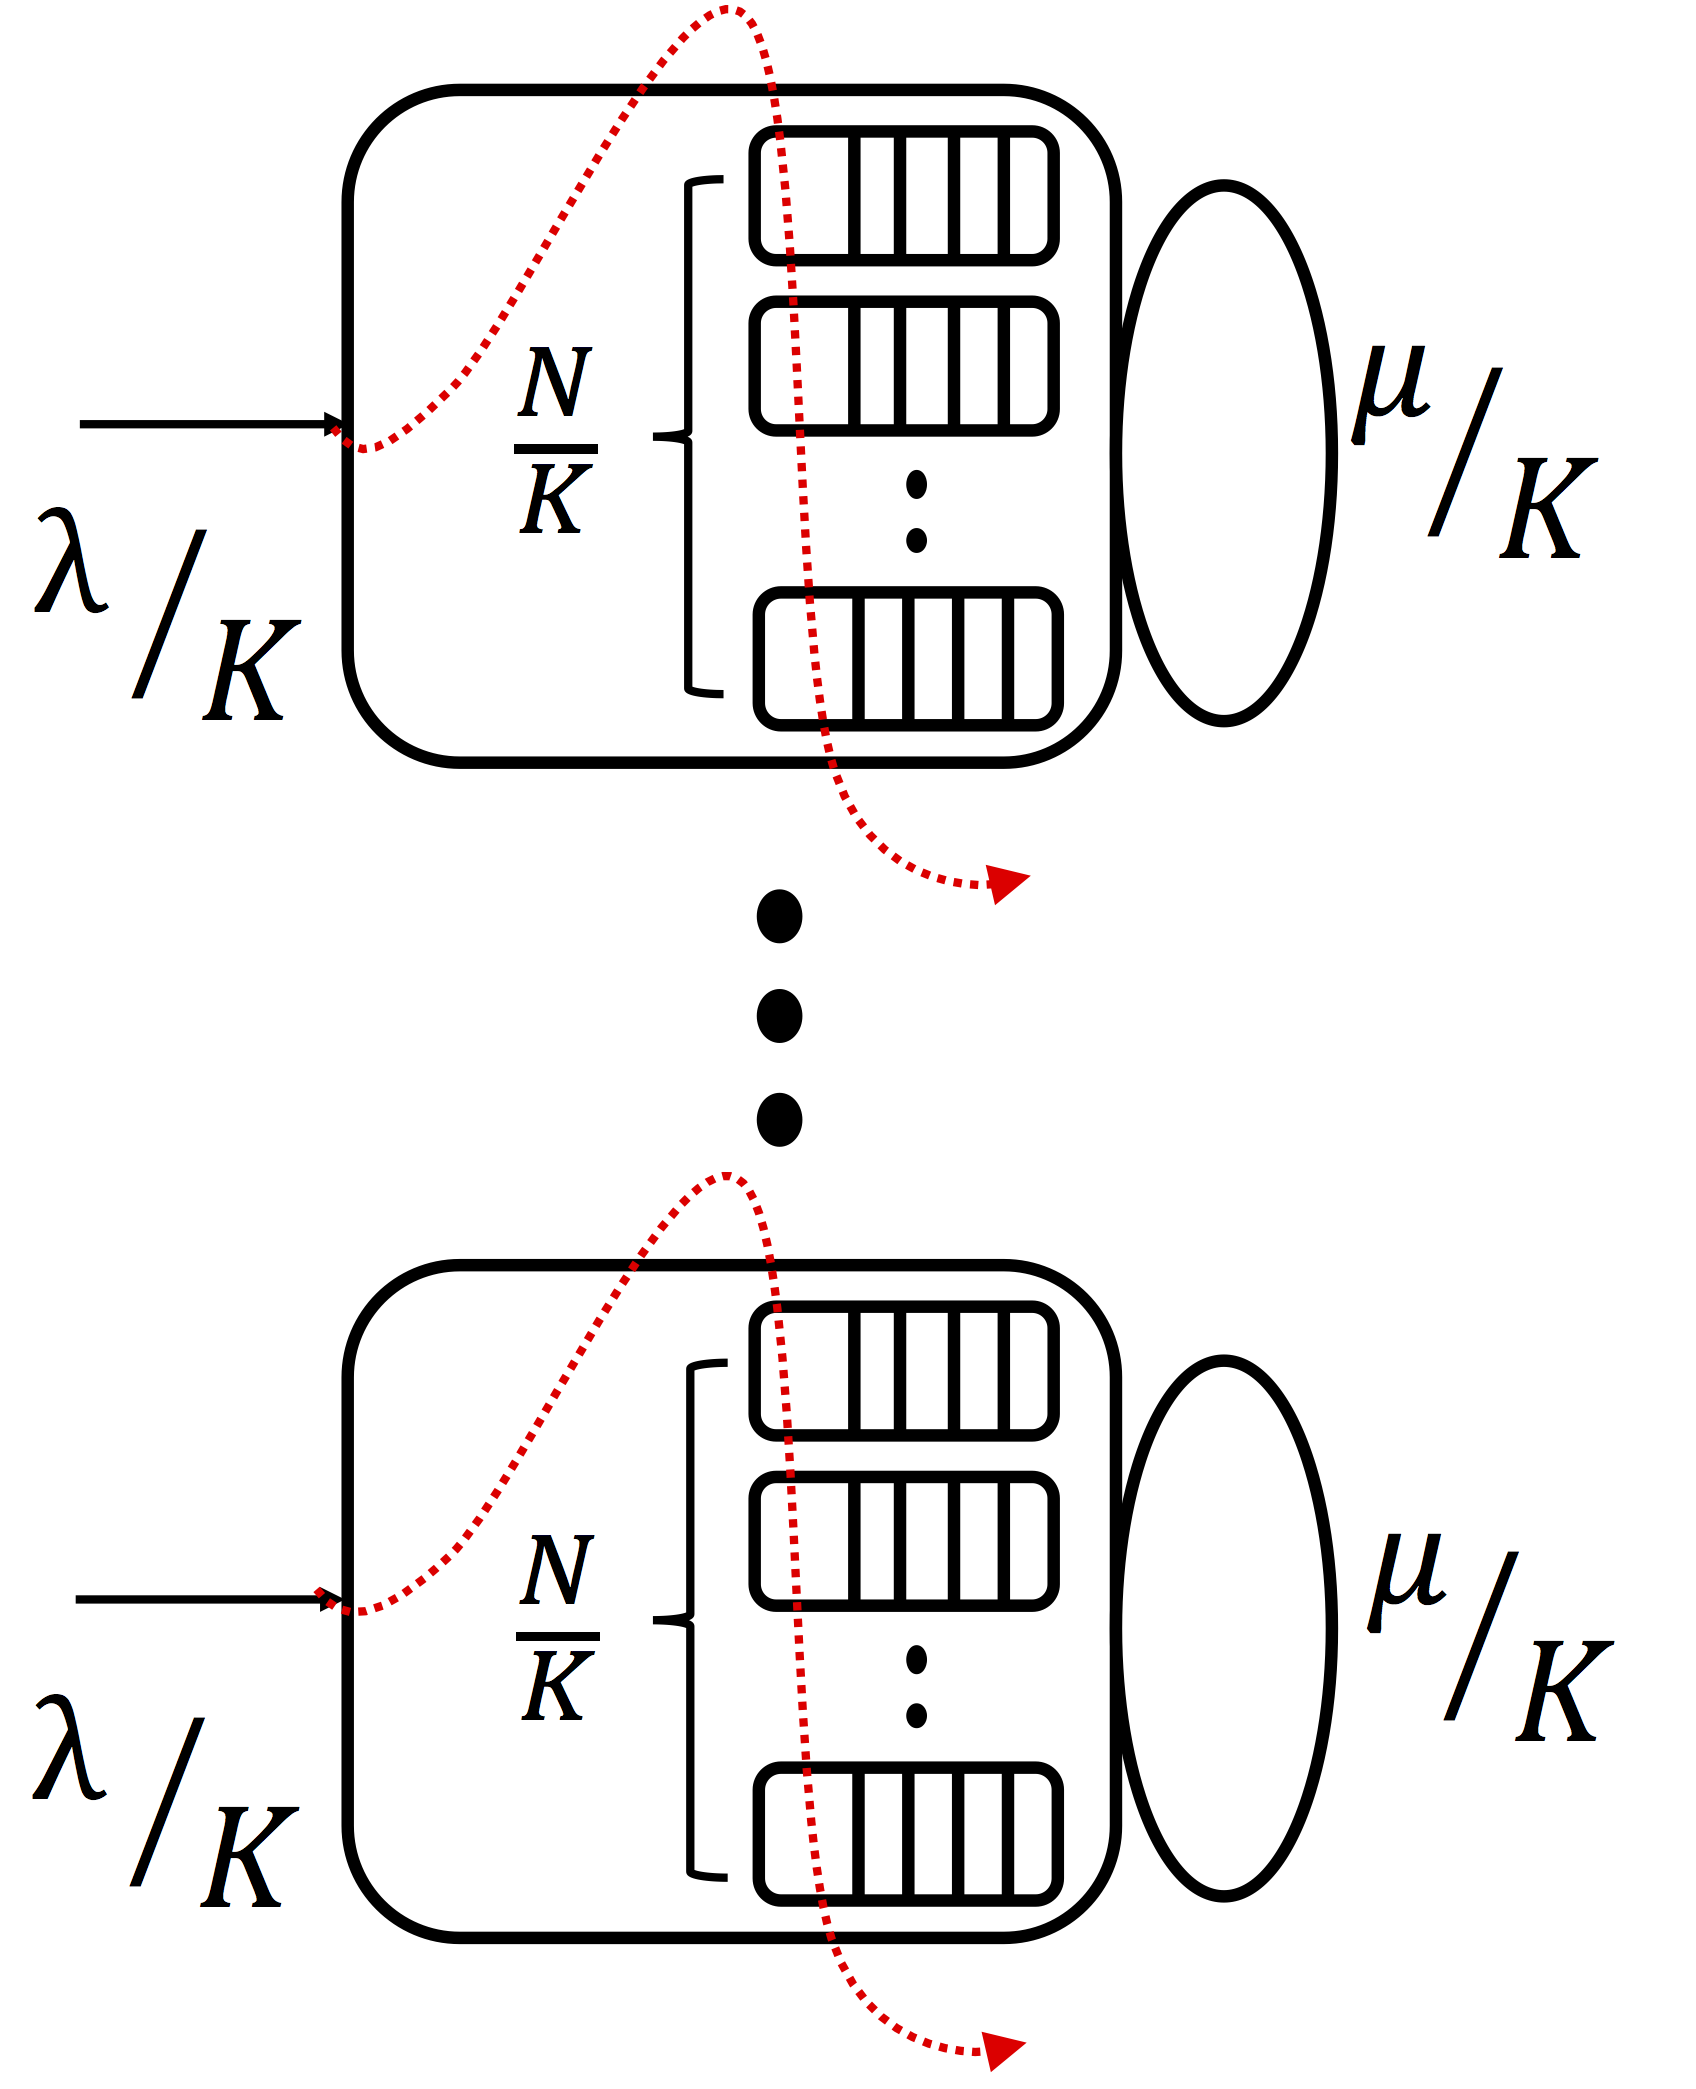
\includegraphics[width=0.8\textwidth]{Chapter3/Figures/esn}
		\caption{Independent servers}
		\label{fig:enn}
	\end{subfigure}
	\hfill
	\begin{subfigure}[b]{0.3\textwidth}
		\centering
		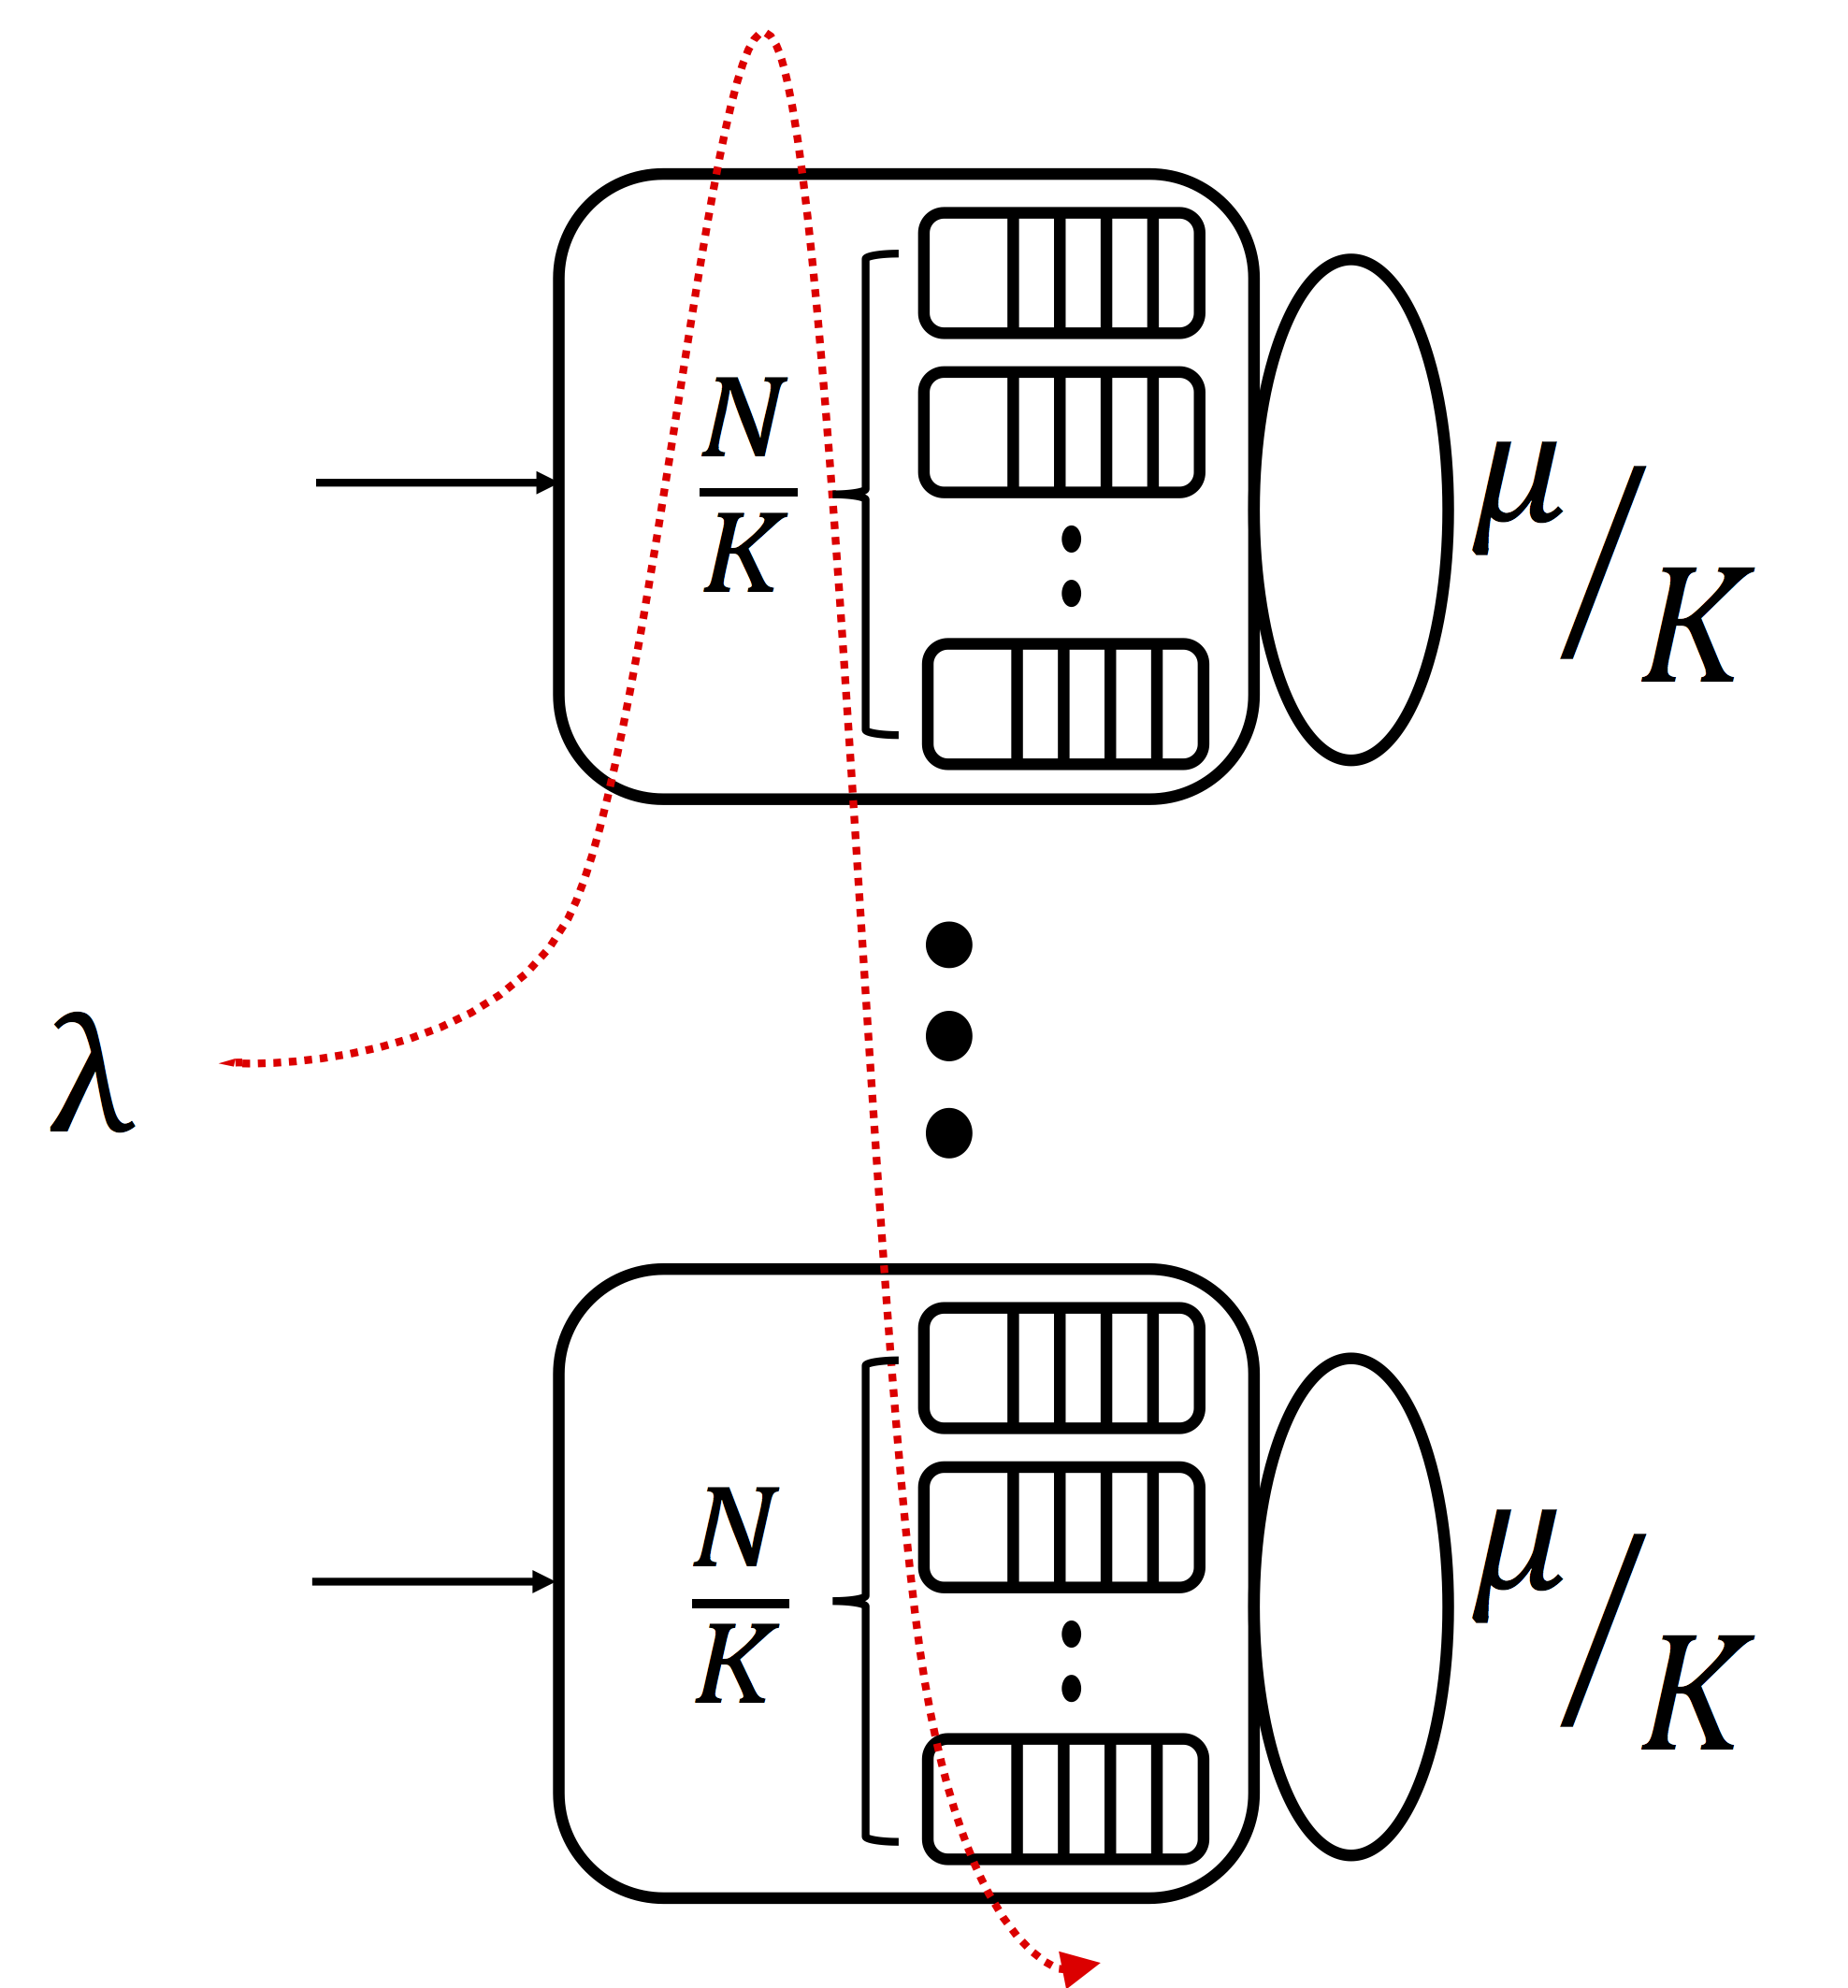
\includegraphics[width=0.9\textwidth]{Chapter3/Figures/sdmlfq}
		\caption{Spatial-diversity}
		\label{fig:sdmlfq}
	\end{subfigure}
	\caption{Three queuing system comparison.} %Red arrows indicate how queues are traversed during flow demotion. On each switch is reported the number of priorities it handles. Color scale is used to emphasize priority levels.}
	\label{fig:three-system-comparison}
\end{figure}
This is an abstraction of the real data center topology. At it heart, a Leaf-and-Spine network with $K$ spines can be described as a queuing system of $K$ parallel G/G/1 servers. Actually, these servers can be equivalently mapped to the \textit{up-send} interfaces that connects a ToR switch to all the spines, as well as to the \textit{down-send} interfaces from different spines to a single ToR. This mapping with the leaf-and-spine topology is shown in Figure \ref{fig:model-dc-map}, where the up-send interfaces are the ones with red texture, whereas the spine down-send interfaces are the ones with light green texture. Ingress and egress ports that connect end hosts to the datacenter network are ignored at this stage. This is in contrast with the data center abstraction provided by pFabric as a giant switch (Figure \ref{fig:pfabricdcn}), where the ingress and egress queues represented the bottleneck where to deploy scheduling strategies, whereas the switching fabric was assumed to be an ideal non-blocking interconnection. Somehow, differently from state-of-the-art solutions that focus only on the bottleneck links assuming that the network is able to sustain maximum throughput with negligible delays, the spatial-diversity approach shifts the attention to the queues inside the fabric itself and rethink the scheduling with a global DC view. Therefore, first it will be assessed the impact of spatial diversity with this simplified model which disregards the hosts and the ingress/egress interfaces, then we will proceed with the implementation on a simulated DCN afterwards.  \\
\begin{figure}
	\centering
	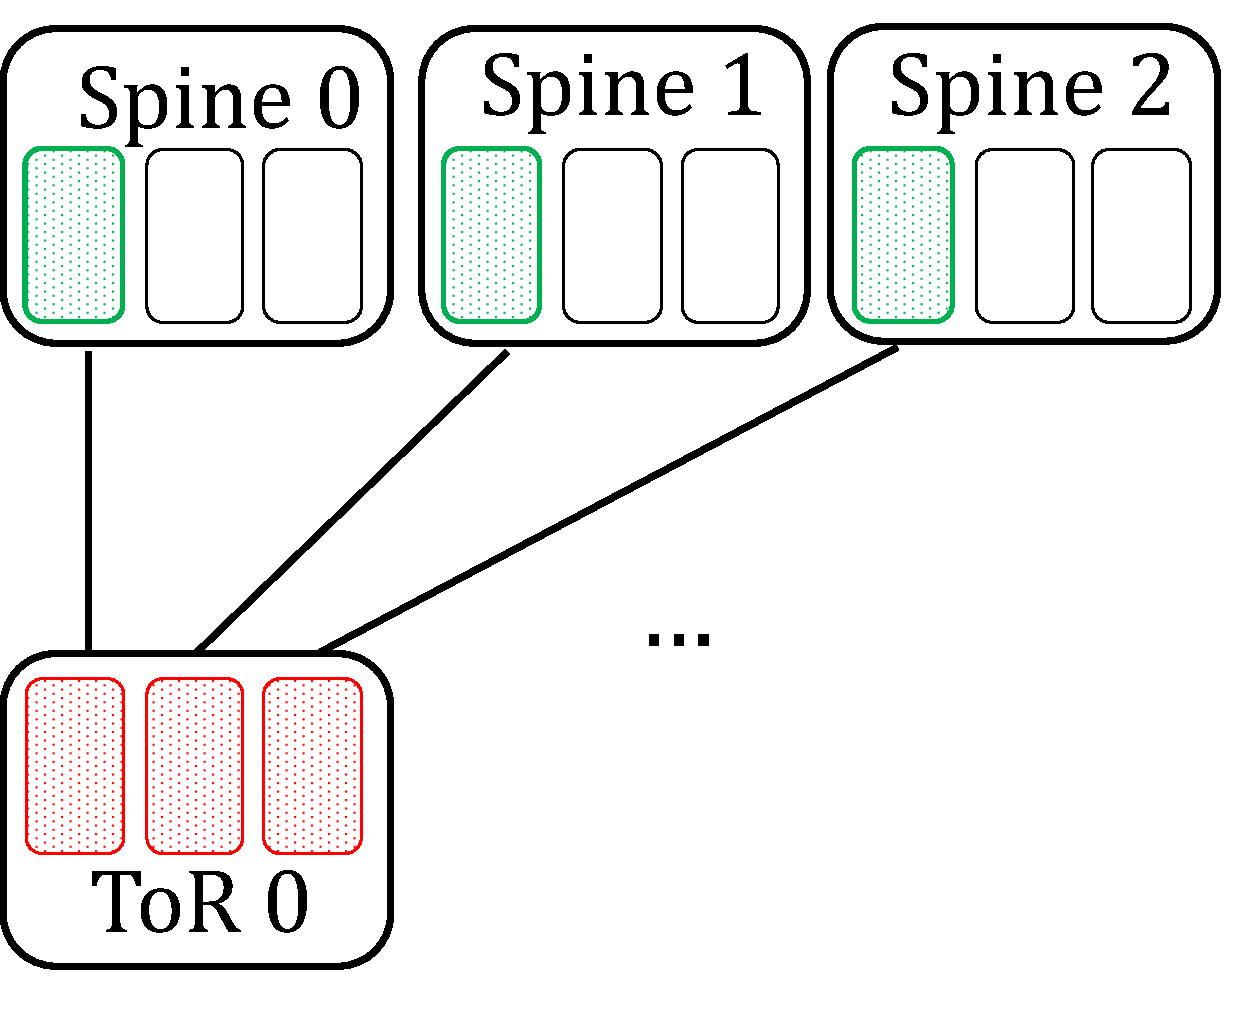
\includegraphics[width=0.3\textwidth]{ChapterSpatialDiversityFramework/Figures/model-dc-map}
	\caption{Mapping of the model abstraction with DCN topology}
	\label{fig:model-dc-map}
\end{figure}
From now on the interfaces considered in the abstract queuing model  of Figure \ref{fig:three-system-comparison} will be interchangeably referred to as servers or spines (with reference to the mapping with down-send spine interfaces).  

The three systems are different alternatives to handle the same total arrival rate $\lambda$ with the same total processing capability $\mu$ and the same number of priority demotion levels $N$. All systems use the mechanism of priority demotion first introduced by PIAS (\S \ref{sec:pias}). Instead, they differ in how priority levels are partitioned on a number $K$ of parallel servers and, more importantly, in the way they use available servers for flow demotion. Specifically, the longest flow that experience all possible demotions follows different trajectory across priority queues and servers. Flow trajectories are represented with dashed red arrows in Figure \ref{fig:three-system-comparison}\\
The first case (Fig. \ref{fig:switchone}) is to have a single high-capacity server that handles all priorities. This of course is the absolute best case where resources are fully concentrated, that provides the smallest delay but does not scale to the dimensions of real systems. It would be equivalent to realize an entire data center interconnection network with a single device of astonishing bandwidth. The second case (Fig. \ref{fig:enn}) is the legacy way to handle priority demotion, where all servers are treated independently in parallel. Flows are evenly load balanced on the available servers and moved across priorities of the same server during their lifetime. In this case the number of demotion levels are limited to \small$\frac{N}{K}$\normalsize. Finally, the third case (Fig. \ref{fig:sdmlfq}) is the novel object we want to investigate, where all the flows are initially sent to the same server, then demoted on the $N$ globally available priority queues. In this case subsequent servers are configured to handle lower and lower priorities, thus part of the flows are re-routed as a consequence of the spatial-diversity. For this reason, in the following of this work also the servers and the links will be labeled as "high priority" or "low priority" for brevity, meaning that they handle high priority traffic or low priority traffic, respectively. 

It was already defined a rigorous mathematical formulation for representing the demotion across priority queues in a single servers as a tandem of M/M/1 queues. (\S. \ref{sec:pias-queueing-model}). The system with spatial diversity introduces a new set of thresholds, which mark the amount of service after which a flow is rerouted to another server. The next section presents a complete formulation for modeling spatial-diversity, starting from the model already defined. 
\section{Mathematical formulation for spatial-diversity}
\label{sec:complete-model}
The introduction of spatial diversity adds a level of complexity to the system. Let's formalize the system setup. There are $K$ parallel servers with $N$ priority queues each one. Thus, there are a total of $K \times N$ priority queues.  All of them are used to add new levels for demotion, therefore flows can assume priority $p \in [1,KN]$ with no duplicate priorities and there are $K \times N - 1$ demotion thresholds. Let's use the variable $j \in [1,K]$ to index the servers and the variable $i \in [1,N]$ to index the priority queues inside each server $s_j$. Starting from the highest level of priority $p$=1 and following descending order of priority up to $p=KN$, the priority levels are assigned to servers from the lower index to the higher index. Thus, server $s_1$ handle priorities $p=\{1,..,N\}$, server $s_2$ handle $p=\{N+1,..,2N\}$, and so on. As in the MLFQ system, whenever a flow at priority $p$ has received service equal to the next threshold, it is downgraded at priority $p+1$. However, differently from MLFQ, it may happen that priority $p$ is assigned to server $s_j$, while $p+1$ is handled by server $s_{j+1}$. In such a case, the flow must be rerouted to a different server. Thus, two related problems need to be solved: finding the set of thresholds that triggers a new flow route from server $s_j$ to server $s_{j+1}$, and finding for each server $s_j$ the set of thresholds that mark the demotion from PQ $i$ to PQ $i+1$, when both PQs are in server $s$. Let's denote them as \emph{load-balance thresholds} and \emph{sub-thresholds}, respectively. 
\smallskip
\begin{tcolorbox}[title=Terminology]
	In a system with priority demotion and with spatial diversity, a flow is moved to a different priority queue (PQ) when the service it has obtained is larger than some threshold. We say that the threshold \textit{push} a flow to a new PQ. We recognize two set of thresholds:
	\begin{itemize}
		\item \textbf{\emph{Load balance thresholds}}. The set of demotion thresholds that push a flow in a priority queue on a server different from the server currently handling the flow itself, implying a flow rerouting.
		\item \textbf{\emph{Sub-thresholds}}. The set of thresholds that push a flow in a different priority queue but in the same server as the one currently handling the flow itself. 
	\end{itemize}
	Correspondingly, we will refer to as:
	\begin{itemize}
		\item \textbf{\emph{Inter-server[spine] demotion.}} A priority demotion involving a load balance threshold.
		\item \textbf{\emph{Intra-server[spine] demotion.}} A priority demotion involving a sub-threshold.
	\end{itemize}
\end{tcolorbox}
\smallskip
The name \emph{load-balance} derive from the fact that the values of these thresholds have strong implications on how the load is distributed across servers. If the thresholds are too small, flows are early rerouted on low priority paths and the capacity of high priority links is essentially wasted. For a real data center implementation this would mean a reduction in the maximum throughput sustained by the switching fabric. As a trivial example, consider a simple topology with two parallel servers each one of normalized capacity 1. In this topology there is only a single threshold that may trigger a flow reroute. With an ideal load balance that evenly distributes the traffic among the two servers, this topology offers a maximum normalized throughput of 2. However, an inappropriate setting of the aforementioned demotion threshold that immediately reroutes flows after negligible attained service would in practice reduce the total capacity  of 50\%. On the other end, still this threshold could be optimal if considering only micro flows, whereas the equal load balance which uniformly splits the traffic on available servers may correspond to a bad demotion threshold for the FCT minimization. In short, a careful tuning of load balance is a new trade-off that was nonexistent in the legacy MLFQ framework, where traffic was demoted to different priority queues but always in the same interface (i.e. link), with zero effects on load balancing. Indeed, a threshold setting that gives an unbalanced load allocation in the available priority queues affects only the delays but not the maximum throughput that the network can sustain. \\
%In SD-MLFQ, depending on the shape of the flow size distribution, latency constrained traffic would either remain unnecessarily mixed with non-demanding latency flows or immediately get.
As concerns the sub-thresholds, they push flows to the same kind of intra-server demotion already studied for MLFQ. However, MLFQ servers work independently and in parallel (Fig. \ref{fig:sd-key-idea-mlfq}) and they are all fed with the same job size distribution. Instead, SD-MLFQ servers observe a different version of the initial workload. Indeed, subsequent servers receive only flows larger than the precedent demotion thresholds, thus they handle truncations of the original flow size distribution above increasing percentiles. As a consequence, while MLFQ thresholds are computed once for all servers, SD-MLFQ sub-thresholds should be optimized depending on the server they belong to. A clarifying overview is provided in Fig. \ref{fig:sd-spine-distribution} for the case of $K$=3 servers $s_1,s_2,s_3$. Figure \ref{fig:wsbp-cdf} is an example job size distribution, from which new flows are randomly generated. In a data center network, this would be the DC-wide workload. On the same axes are drawn the two example split thresholds, denoting the amount of service in kilobytes after which a flow is rerouted from $s_1$ to $s_2$ and then from $s_2$ to $s_3$. 
\begin{figure}
	\centering
	\captionsetup{width=.8\linewidth}
	\begin{subfigure}{.3\textwidth}
		\centering
		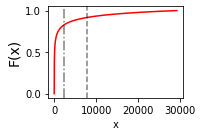
\includegraphics[width=1.05\textwidth]{Chapter3/Figures/ws-bp-cdf}
		\caption{Workload on $s_1$}
		\label{fig:wsbp-cdf}
	\end{subfigure}%
	\hfill
	\begin{subfigure}{.3\textwidth}
		\centering
		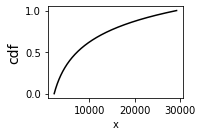
\includegraphics[width=\textwidth]{Chapter3/Figures/wsbp-highp-cdf}
		\caption{Workload on $s_2$}
		\label{fig:highp-cdf}
	\end{subfigure}
	\hfill
	\begin{subfigure}{.3\textwidth}
		\centering
		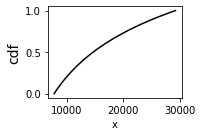
\includegraphics[width=\textwidth]{Chapter3/Figures/wsbp-lowp-cdf}
		\caption{Workload on $s_3$}
		\label{fig:lowp-cdf}
	\end{subfigure}
	\caption{Job size distributions observed by servers $s_1$, $s_2$, $s_3$ in decreasing order of priority. Optimal load balance split for $\lambda=0.9$.}
	\label{fig:sd-spine-distribution}
\end{figure}
Since all flows enter the system through $s_1$, this distribution is also the one observed by the highest priority server $s_1$. Then, subsequent servers of lower priorities observe left-truncated versions of the initial workload on $s_1$. 


An intuitive solution to address both load balance thresholds and sub-thresholds at once is to write an extension to the PIAS model that embeds spatial-diversity. This formulation, explained in details below, would in principle guarantee optimal performances. Indeed, it jointly captures in a unique model all the dynamics of the system.
\subsubsection{Optimal solution}
The optimization problem Eq.\eqref{eq::costfunction} can be extended to the case of spatial diversity.
Assume the capacity of a single server to be $\mu/K$, so that the total capacity is always $\mu$. All the servers work independently with same rate $\mu / K$. Still there is a SP scheduler orchestrating priority queues in every server, but there is no coordination among different servers, meaning that there is not a global SP scheduler to discipline the transmission among distinct servers. Indeed, such a tight control among physically different devices would be almost impossible to realize in practice, at least packet by packet. \\
Let the notation $\mu_i^j$ indicate the drain rate of the $i$-th queue in the $j$-th server $s_j$ $(1 \le i \le N, 1 \le j \le K)$, and equivalently use $\lambda_i^j$ for the arrival intensities and in general the superscript $j$ for any quantity already defined for the queues in the basic model in Sec.\ref{sec:pias-queueing-model} but applied to queues inside server $s_j$. A summary of all the quantities involved in the queuing model is found in Table $\ref{tab:queuingmodel}$. It follows:
\begin{align*}
\lambda_i^j &= \lambda \mathbb{E}[L_i^j] \\
\mu_i^j &=  \dfrac{\mu}{K} \prod_{l=1}^{i-1}(1-\rho_l^j) \\
\theta_i^j &= F(\alpha_i^j) - F(\alpha_{i-1}^j)	\\
\mathbb{E}[T_i^j] &= \dfrac{1}{\mu_i^j - \lambda_i^j}
\end{align*}
The formulation is essentially the same but with an additional dimension that takes into account the existence of multiple servers. Every server is modeled as a tandem of $N$ queues, exactly as in PIAS. Then, there are $K$ of them in parallel. Also, we wrote an additional constraint Eq.\eqref{eq:overload-constr} that prevents overloading any spine 
\textcolor{red}{(TODO: additional constraint is it really needed??? in case of overloading, sojourn times goes to infinity, so it is unlikely it is chosen as solution....)}. 
\begin{subequations}
	\begin{align}
	&\underset{\{\theta_i^j\}}{\text{min}} & \quad  & \mathcal{T} =	\sum_{j=1}^{K}\sum_{i=1}^{N} \theta_i^j \sum_{j=i}^{N}T^s_j 					\label{eq::costfunction-spatial} & \\
	&\text{subject to} & \quad  &\theta_i^s \ge 0 & \\
	& & & \sum_{i=1}^{N} \theta_i^j = 1  \qquad \forall j \in [1,K] &  \\
	& & & \sum_{i=1}^{N}  \lambda_i^j < \mu/K  \qquad \forall j \in [1,K] & \label{eq:overload-constr}
	\end{align}
	
\end{subequations}
This approach would provide optimal load balancing and at the same time would choose a set of sub-thresholds targeted on the optimal load balance thresholds. Notably, the optimal solution would never include load balance thresholds that lead to an unbalanced traffic distribution among the servers, because that would have an overkilling effect on the delays, which instead the problem tries to minimize. Despite being a clean analytical formulation, its complexity seems prohibitive. The basic model without spatial diversity yet was non-convex and presented products and ratios of variables (Sec. \ref{sec:pias-queueing-model}). Nonetheless, it is still tractable since the number of variables is typically bounded to the (low) number of PQs available in commodity switches. Instead, in the complete model the number of variables scales with the product $K \times N$, where $K$ is usually big for large-scale data centers. In the next chapter we will provide in more details the CPU-time spent by two well-known meta-heuristics solvers, specifically PSO \cite{pso,pso2} and Basin-Hoppin \cite{basinhoppin} before to converge. Anyway, if the time scale at which a solution could be found is excessively large, the system would be unable to react promptly to a sudden change of the flow size distribution. As a consequence, the system would operate for long using thresholds mismatched with respect to the flow distribution. Therefore, even finding an optimal solution once does not signify that this approach is feasible for a real datacenter scenario, where likely the solution must be computed repeatedly as statistics change. \\
To the purpose of investigating the spatial diversity framework, it has been preferred to handle the two problems individually. The approach that has been carried out is decoupled in two sequential steps.
\begin{enumerate}
	\item \textbf{Optimize load-balance thresholds.} First it is solved an optimization problem with the goal of finding the best load partitioning among $K$ servers. Servers are always assumed to have a single priority ($N$=1), because for the time being sub-thresholds are ignored. At the end of this phase a set of $K$-1 load balance thresholds is delivered.
	\item \textbf{Greedy subthresholds}. The load-balance thresholds are provided as input of the second phase. They split the support of the flow size in $K$ disjoint intervals covering the whole support. The $i$-th interval contains the sizes of those flows that end their service in server of priority $i$. On each interval is computed a set of sub-thresholds with a greedy algorithm like ES-N or LS-N, but applied to the truncated distributions (Sec.\ref{sec:greedy-thresh}).  
	%Each of them truncates the original flow size distribution at a given percentile. 
\end{enumerate}

\subsection{Decouple load balance from sub-thresholds}
\label{sec:decoupling}
\subsubsection{Optimize load balance thresholds}
\label{sec:optimal-lb-problem}
For the first phase turns out again to be useful the stochastic queuing model of MLFQ as provided in PIAS. (Sec.\ref{sec:pias-queueing-model}-Fig.\ref{fig:pias_scheme}). Each server is equipped with a single priority queue per port, therefore the optimal load balance problem can be abstracted with exactly the same model, where each queue in the tandem maps a server. After all, in this case priority queues are physically distributed to different servers, instead of being part of the same interface. They are independent on each other and the strict priority scheduler is no more involved, as they work in parallel without coordination. Practically, the only modification is to the queues capacities $\mu_i$. Remember that in the aforementioned MLFQ model the strict priority scheduler was described by attenuating the PQ serving rates $\mu_i = \mu\prod_{i}(1-\rho_i)$ for increasing $i$. Because of servers work in parallel without scheduling, this expression is not needed anymore and the draining rates just coincide to the same value:
\[
\mu_i = \mu \mslash K, \qquad i=1,..,K
\]
% TODO Keep in mind that these are just the flow size distributions and not the actual traffic handled by a server. For example, $s_0$ serve only the first $\Omega_1$ bytes of all flows, including those larger than $\Omega_1$ . The actual byte arrivals were obtained with Eq.\eqref{load-on-pqi}, that does require these distributions to be known.
\subsubsection{Choose greedy sub-thresholds}
\label{sec:subthresh-with-sd}
Lastly, it is addressed the problem of finding the sub-thresholds. Starting from the optimal load balance thresholds that have been found in the previous step, each server is then treated individually. Remember that whatever policy is adopted for sub-thresholds computation, it has to be applied to all servers individually, since they observe different flow size distributions. All the threshold computation algorithms defined so far (\S \ref{sec:pias-queueing-model}, \S \ref{sec:greedy-thresh}) require the knowledge of the flow size distribution. It is pretty straightforward to obtain the p.d.f. $f(x)$ and the corresponding c.d.f. $F(x)$ as distribution conditioned to the truncated supports. There are $K$ servers and $K-1$ load balance thresholds. For the sake of conciseness, denote the load balance thresholds $\alpha_N^j$ which triggers a flow reroute from server $j$ to server $j+1$ as $\Omega_j$. On server $j$ the initial distribution is normalized on a new support $[\Omega_{j-1},\infty)$. Thus, from probability theory:
\begin{equation}
\label{eq:conditionalpdf}
\begin{aligned}
F(x|x>\Omega_{j-1}) &= \dfrac{F(x) - F(\Omega_{j-1})}{1-F(\Omega_{j-1})}  \\
f(x|x>\Omega_{j-1}) &= \dfrac{f(x)}{1-F(\Omega_{j-1})} 
\end{aligned}
\end{equation}
Once these distributions are known, nothing is missing to apply the greedy sub-threshold assignment algorithms depicted in Sec. \ref{sec:greedy-thresh}. For completeness, they are briefly rewritten under this framework. Define in short:
\begin{align*}
f_T(x) =& f(x|x>\Omega_{j-1})\\
\bar{F}_T(x) =& \bar{F}(x|x>\Omega_{j-1}). 
\end{align*}
Enumerate the available server $s \in \{1,..,K\}$. The goal is to find on all servers a set of sub-thresholds $\alpha_i^s$ to delimit demotion bounds across priority queues $i \in \{1,..,N\}$. \\
\textit{Equal-Split-N} (ES-N) is substantially the same:
\begin{equation}
\alpha_i^j = F_T^{-1}\Big(\frac{i}{N}\Big)
\end{equation}
\textit{Load-Split-N} (LS-N) is also very similar. It required the solution of the set of load balance equations \ref{eq:main-K-PQ}. The expression of the average traffic $\mathbb{E}[L_i^j]$ on priority $i$ of server $s_j$ is unchanged. However, additional care must be paid to their sum $\sum_{i=1}^{N}\mathbb{E}[L_i^j]$. From proof \ref{proof}, this sum was equal to:
\[
\sum_{i=1}^{N}\mathbb{E}[L_i^j] = \int_{\Omega_{j-1}}^{\Omega_j}xf_T(x)dx + \Omega_{j} \bar{F}_T(\Omega_{j}) -\Omega_{j-1}\bar{F}_T(\Omega_{j-1})
\]
and the terms outside the integral always amounted to zero, so that the sum gave $\int_{\Omega_{j-1}}^{\Omega_j}xf_T(x)dx = \mathbb{E}[X]$. Instead, in this case they are generally different zero because the lower threshold $\alpha_0^j = \Omega_{j-1} \neq 0$ and the survival function above the upper threshold $\bar{F}_T(\alpha_N^j) = \bar{F}_T(\Omega_j) \neq 0$. Everything else is the same.
\\

As already mentioned, it is very likely that this approach is sub-optimal. However, it represents an handful way of computing all the thresholds in order to establish some understanding about the integration of spatial diversity with an MLFQ system. 